\documentclass[a4paper,11pt,titlepage]{jsarticle}
\usepackage[final]{graphicx}
\usepackage[dvipdfmx]{color}
\usepackage{listings, xcolor}
\usepackage{amsmath}
\usepackage{here}

\lstset{
  basicstyle=\footnotesize\ttfamily,
  frame=tbrl,
  breaklines=true,
  numbers=left,
  keywordstyle=\color{blue},
  commentstyle=\color[HTML]{1AB91A},
  stringstyle=\color{brown},
  captionpos=t
}

\title{機械学習 課題:学習定数を定める}
\author{235738B 越後 玲輝}

\begin{document}

\maketitle

\section*{1. 課題概要}
textのAdalineのコードを実行して、学習定数の値をさまざまに試し、最適と思われる値を特定してください。  
また、その値を選んだ理由も添えてください。

\section*{2. Pythonコード}
\lstinputlisting[caption=Adaline学習率比較コード, language=Python]{adaline_rep1.py}

\section*{3. 実験結果}
以下の図は、各学習率ごとの平均コスト(SSE: Sum of Squared Errors)の変化を示している。

\begin{figure}[H]
    \centering
    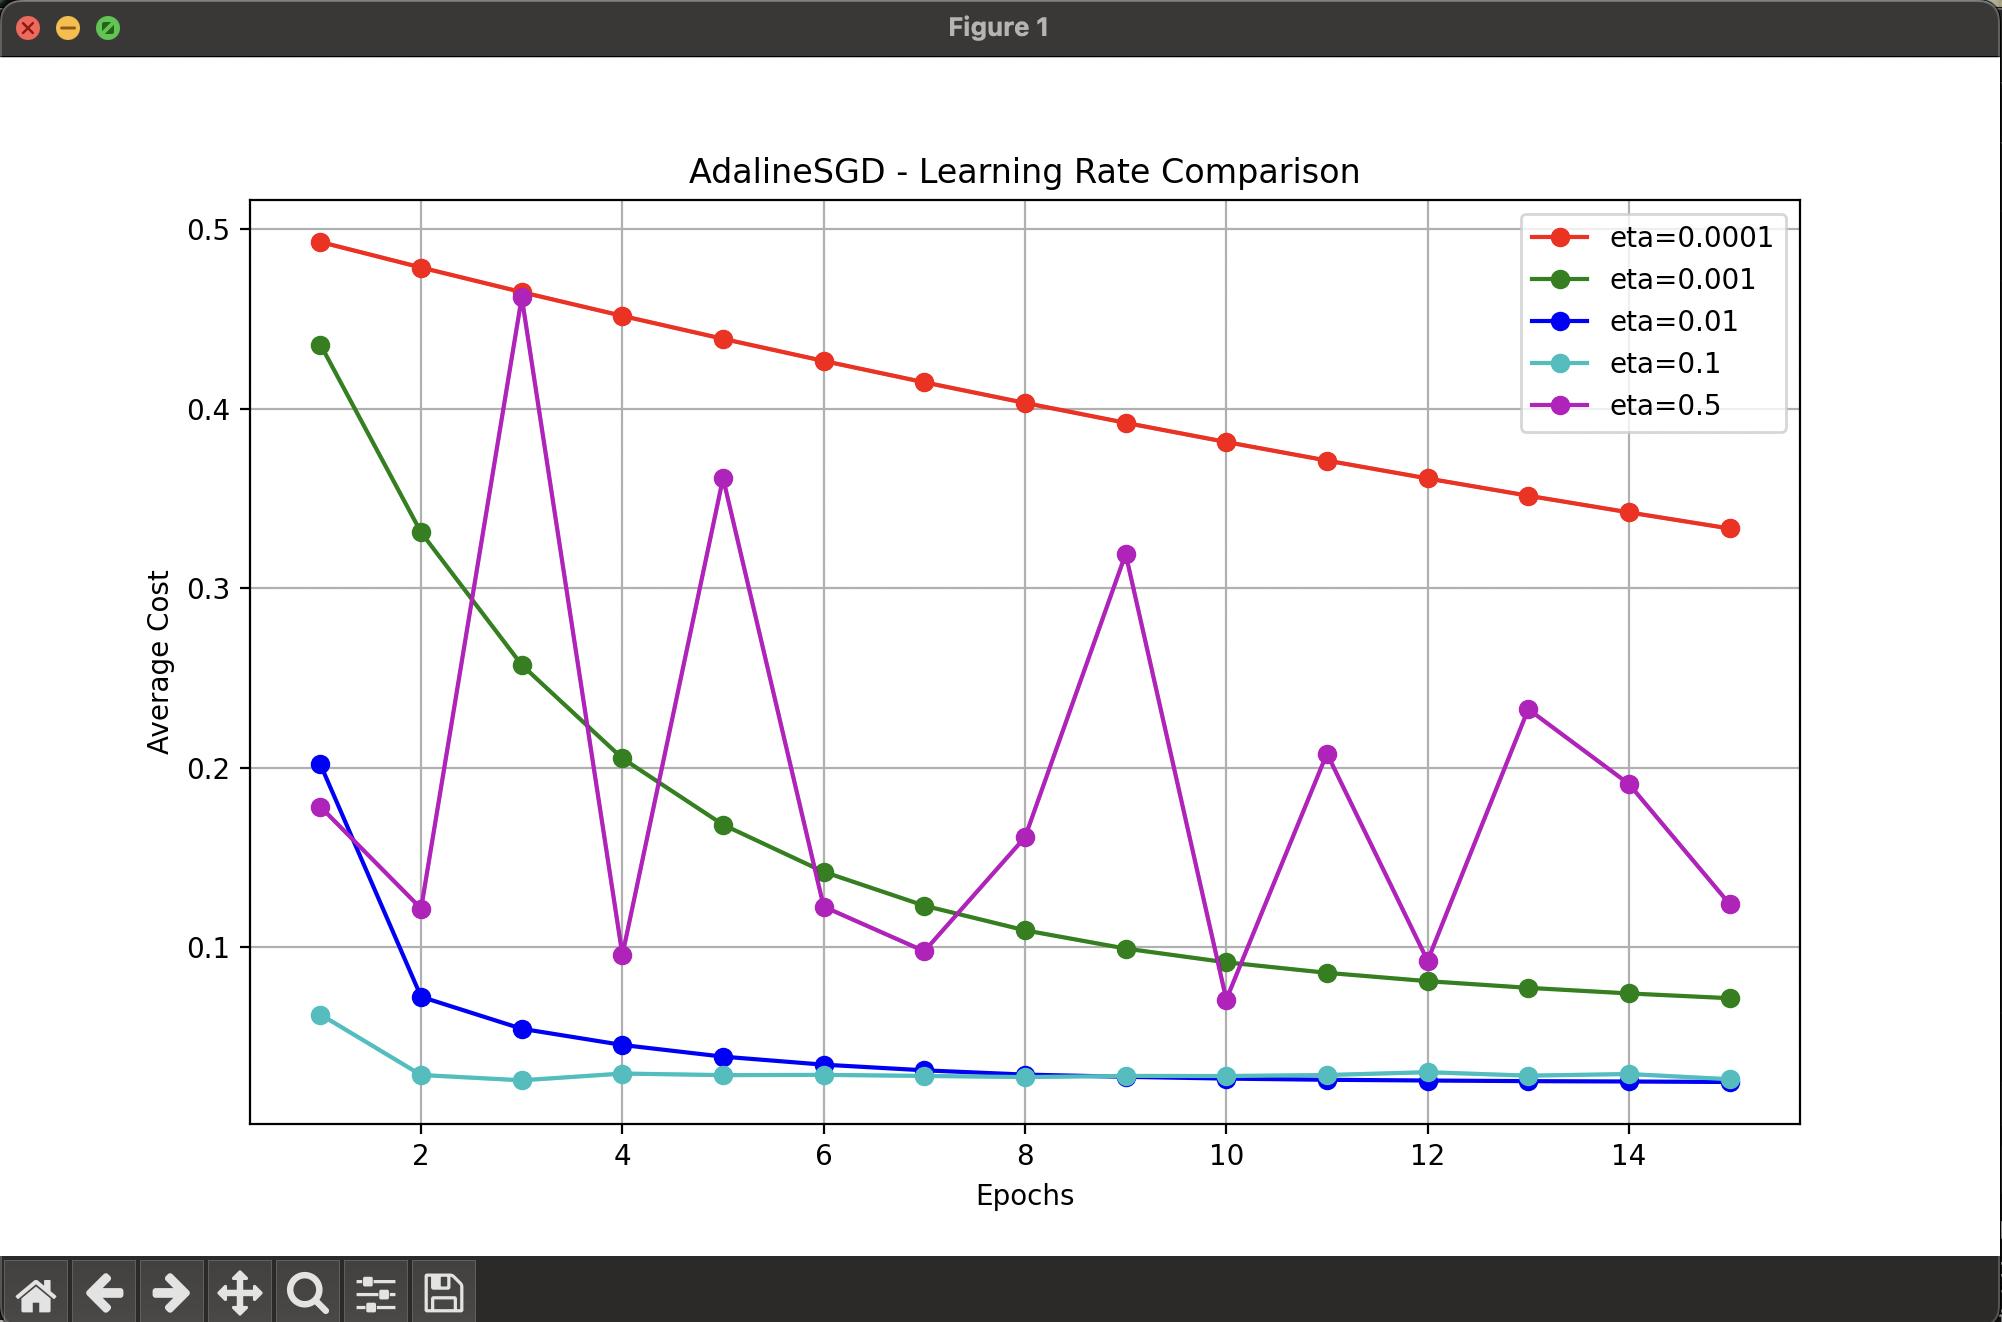
\includegraphics[width=0.8\linewidth]{eta_comparison.png}
    \caption{学習率ごとの平均コスト推移(AdalineSGD)}
\end{figure}

グラフの描画には、Pythonライブラリである\texttt{matplotlib.pyplot}を用いた。  

各学習率($\eta$)ごとに15エポックの学習を実行し、各エポックの平均コスト(SSE)をリストとして記録。
  
エポック数を横軸、平均コストを縦軸として描画。 

\section*{4. 各学習率について考察}

それぞれの学習率に対して、以下のような学習挙動が見られた。

\begin{itemize}
    \item \textbf{$\eta = 0.0001$:} 学習率が極めて小さいため、1回の更新による重みの変化が微小となり、学習が進みにくく、結果として収束に非常に時間がかかる。
    
    \item \textbf{$\eta = 0.001$:} 多少改善されたものの、更新幅が小さく、依然として誤差の減少速度は遅い。精度は上がるが効率は悪い。
    
    \item \textbf{$\eta = 0.01$:} 重みが過不足なく更新されるため、誤差が安定して減少し、効率よく収束するパターン。
    
    \item \textbf{$\eta = 0.1$:} 学習率がやや大きいため、収束は速く見えるものの、最適値の周囲でコストにブレを確認。
        
    \item \textbf{$\eta = 0.5$:} 学習率が大きすぎて、重みが極端に更新されることで適切な方向に学習が進まず、むしろ誤差が増加する傾向となった。
\end{itemize}

これらの結果から、学習率は小さすぎても大きすぎても学習が非効率・不安定となるため、$\eta = 0.01$ のような中間的な値が最も望ましいといえる。


\section*{5. 結論}
$\eta$を $0.0001$ から $0.5$ まで5段階で変化させた。
それぞれの学習率について平均コストの推移を観察した結果、$\eta = 0.01$ のときに最も安定して学習が進み、15エポック以内に誤差が十分に収束した。これに対して、$\eta = 0.0001$ や $0.001$ では収束が遅く、$\eta = 0.1$ 以上では誤差が発散または振動する傾向が見られた。したがって、$\eta = 0.01$ が最もバランスの取れた学習定数であり、最適であると判断した。

\end{document}
